%%%%%%%%%%%%%%%%%%%%%%%%%%%%%%%%%%%%%%%%%%%%%%%%%%%%%%%%%%%%%%%%%%%%%%%%%%%%%%%%
%% DAS PE4 -- SQL Injection with Protection (More than 1 variant)
%% Springer Nature LaTeX template (sn-jnl).
%%
%% HOW TO USE (Overleaf):
%%   1. Open the "Springer Nature LaTeX Template" on Overleaf (menu:
%%      New Project -> Templates -> search "Springer Nature").
%%   2. Replace the template's main.tex with THIS file.
%%   3. Upload references.bib and the figures/ folder (5 PNGs) into the project.
%%   4. Set the compiler to pdfLaTeX and click Recompile.
%%
%% The class file sn-jnl.cls and the .bst files ship with that template, so do
%% NOT copy them from here -- only this main.tex, references.bib, and figures/.
%%%%%%%%%%%%%%%%%%%%%%%%%%%%%%%%%%%%%%%%%%%%%%%%%%%%%%%%%%%%%%%%%%%%%%%%%%%%%%%%

\documentclass[pdflatex,sn-mathphys-num]{sn-jnl}

%% Packages that are safe alongside the Springer Nature class
\usepackage{graphicx}
\usepackage{multirow}
\usepackage{amsmath,amssymb,amsfonts}
\usepackage{booktabs}
\usepackage{url}
\usepackage[T1]{fontenc}
\usepackage{listings}
\usepackage{xcolor}
\usepackage{tikz}
\usetikzlibrary{positioning,arrows.meta,shapes.geometric}

\graphicspath{{figures/}}

% Listing style for SQL / payloads
\definecolor{codebg}{RGB}{245,246,248}
\definecolor{codekw}{RGB}{30,80,200}
\lstset{
  basicstyle=\ttfamily\footnotesize,
  backgroundcolor=\color{codebg},
  breaklines=true,
  frame=single,
  columns=fullflexible,
  keepspaces=true,
  showstringspaces=false
}

\raggedbottom

\begin{document}

\title[SQL Injection with Protection]{SQL Injection with Protection: A Defence-in-Depth Study and Multi-Variant Live Prototype}

\author*[1]{\fnm{YashVardhan} \sur{Gupta}}\email{yashvardhan3.mitmpl2023@learner.manipal.edu}
\author[1]{\fnm{Sheldon} \sur{Rodricks}}\email{sheldon.mitmpl2023@learner.manipal.edu}
\author[1]{\fnm{Lakshya} \sur{Agrawal}}\email{lakshya3.mitmpl2023@learner.manipal.edu}
\author[1]{\fnm{Aditya Aryan} \sur{Sahu}}\email{aditya9.mitmpl2023@learner.manipal.edu}

\affil[1]{\orgdiv{Department of Computer Science and Engineering},
  \orgname{Manipal Institute of Technology, Manipal Academy of Higher Education},
  \orgaddress{\city{Manipal}, \state{Karnataka}, \country{India}}}

\affil{\textit{Registration numbers:} YashVardhan Gupta (230905442),
  Sheldon Rodricks (230905324), Lakshya Agrawal (230905552),
  Aditya Aryan Sahu (230905560)}

\abstract{Structured Query Language injection (SQLi) has remained in the OWASP
Top-10 injection category for over a decade because its root cause---the
confusion of untrusted \emph{data} with executable \emph{code}---recurs wherever
input is concatenated into a query. This paper surveys ten peer-reviewed studies
published between 2023 and 2026 and shows that the field has largely solved
\emph{offline} detection (reported accuracies of 0.94--0.99) while leaving open
gaps in adversarial robustness, generalization, and deployable prevention. Guided
by these gaps, we design and evaluate a defence-in-depth login application that
implements five protection variants---parameterized queries, allow-list input
validation, object--relational mapping (ORM), salted credential hashing, and a
transparent signature web-application firewall (WAF)---against a common battery
of tautology, comment, and UNION payloads. On our reproducible testbed the
vulnerable baseline is bypassed by a single-line payload, whereas every
protection variant blocks the identical payload while preserving legitimate
authentication, at a measured query cost below one millisecond. The prototype
converts the surveyed gaps into a concrete, testable artefact and frames adaptive,
adversarially robust detection as the next layer of defence.}

\keywords{SQL injection, web application security, parameterized queries, input
validation, web application firewall, defence in depth}

\maketitle

%%======================================================================%%
\section{Introduction}\label{sec:intro}

Web applications mediate access to the databases that hold an organization's most
sensitive records, and Structured Query Language injection (SQLi) is the archetypal
attack against that boundary. An SQLi vulnerability exists whenever attacker-controlled
input is placed into a query string that the database then parses as code; a single
crafted value such as \lstinline|' OR '1'='1' -- | can then subvert the query's
logic to bypass authentication, read arbitrary rows, or modify data. Despite being
well understood for more than twenty years, injection remains ranked in the OWASP
Top-10~\cite{owasp2021top10}, and recent work confirms that even commercial
defences are routinely bypassable~\cite{qu2024advsqli}.

The persistence of SQLi is not due to a lack of countermeasures but to their uneven
application and to an arms race with increasingly sophisticated evasion. Protection
spans two families. \emph{Secure-coding} controls---parameterized queries, allow-list
input validation, ORM-mediated access, least-privilege database accounts, and salted
password hashing---eliminate the code/data confusion at the source. \emph{Runtime}
controls---signature- and learning-based web-application firewalls (WAFs) and
network-flow monitors---observe traffic and block malicious requests. A central
theme of the recent literature, and of this paper, is that no single control is
sufficient: robust protection is \emph{layered}.

This paper makes three contributions. First, it surveys ten studies from 2023--2026
(Section~\ref{sec:survey}) and distils four open research gaps
(Section~\ref{sec:gap}). Second, it designs a defence-in-depth login application
that realises five protection variants around a common data model
(Section~\ref{sec:method}). Third, it evaluates the variants against a shared
payload battery and reports both security outcomes and query-time cost
(Section~\ref{sec:eval}). All code, payloads, and screenshots are released as a
reproducible prototype for teaching and demonstration.

\section{Background}\label{sec:background}

\subsection{Anatomy of a SQL injection}
Consider a login handler that builds a query by concatenation:
\begin{lstlisting}[language=SQL]
SELECT id, role FROM users
WHERE username = '<user>' AND password = '<pass>';
\end{lstlisting}
If \verb|<user>| is set to \lstinline|admin' -- |, the trailing \verb|-- | comments
out the password check and the interpreter executes
\lstinline|... WHERE username = 'admin'|, authenticating the attacker as
\texttt{admin}. Variants include boolean \emph{tautologies}
(\lstinline|' OR '1'='1|), \emph{UNION}-based data exfiltration, \emph{stacked}
queries, and \emph{blind} time-based inference. What unifies them is that the input
crosses the boundary from data into query syntax.

\subsection{Taxonomy of protections}
Table~\ref{tab:taxonomy} summarises the controls evaluated in this work and where
each intervenes. The design principle is defence in depth: an attacker must defeat
every layer, whereas the defender benefits from any one holding.

\begin{table}[htbp]
\caption{Protection variants implemented in the prototype and their point of intervention.}\label{tab:taxonomy}
\begin{tabular}{@{}p{3.1cm}p{5.6cm}p{3.2cm}@{}}
\toprule
Variant & Mechanism & Intervenes at \\
\midrule
Parameterized query & Input bound as a typed parameter; never parsed as SQL & Database driver \\
Allow-list validation & Accept only characters valid for the field; reject early & Application input \\
ORM & Query built from objects; parameterization by construction & Data-access layer \\
Credential hashing & Salted one-way hash; lookup by username then verify & Credential store \\
Signature WAF & Regex/heuristic inspection of requests before execution & Request gateway \\
\bottomrule
\end{tabular}
\end{table}

\section{Literature Survey (2023--2026)}\label{sec:survey}

Following the departmental convention, each study's methodology is described in the
past tense and its remaining limitation in the present tense.

\paragraph{Crespo-Mart\'inez et al. (2023)}
addressed the impracticality of inspecting every packet for SQLi on
heavily loaded routers~\cite{crespo2023sqli}. The authors gathered two datasets of
network-flow records from SQLi attacks against popular database engines and
evaluated several machine-learning algorithms, selecting a logistic-regression
model. They reported a detection rate above 97\% with a false-alarm rate below
0.07\% using flow data alone. The method is limited by its reliance on coarse
flow-level features, which omit the query payload and constrain detection of
obfuscated variants.

\paragraph{Alghawazi, Alghazzawi and Alarifi (2023)}
studied deep sequence learning for SQLi text~\cite{alghawazi2023rnn}. They trained a
recurrent-neural-network autoencoder on a public dataset of benign and malicious
statements and benchmarked it against seven conventional classifiers, reporting 94\%
accuracy and a 92\% F1-score. The method is limited by a moderate accuracy ceiling
and single-corpus evaluation, leaving real-world generalization uncertain.

\paragraph{Thalji et al. (2023)}
automated feature engineering with an autoencoder network,
``AE-Net''~\cite{thalji2023aenet}. Using a preprocessed corpus of 46{,}392 queries,
they learned deep features fed to several classifiers and validated with k-fold
cross-validation and a t-test; an extreme gradient-boosting model reached 0.99
accuracy. The approach is limited by evaluation on a curated dataset without
real-time or adversarial testing.

\paragraph{Alotaibi and Vassilakis (2023)}
implemented a web-application firewall inside a software-defined-networking (SDN)
controller~\cite{alotaibi2023sdnwaf}. They combined signature and regular-expression
detection and compared the system with ModSecurity, showing successful blocking and
lower TCP-ACK latency. The design is limited by signature/regex matching that does
not generalize to unseen payloads and by the centralized controller as a bottleneck.

\paragraph{Arasteh et al. (2024)}
framed detection as feature selection~\cite{arasteh2024graywolf}. They prepared a
13-feature dataset and developed two binary gray-wolf optimizers to select the most
informative subset for several classifiers, reporting 99.68\% accuracy while using
about 20\% of features. The method is limited by the search cost and initialization
sensitivity of the metaheuristic and by single-dataset validation.

\paragraph{Paul, Sharma and Olukoya (2024)}
argued that prior work ignores prioritization and prevention~\cite{paul2024sqlreaper}.
From 457{,}233 traffic samples (70{,}023 with SQLi payloads) they built
``SQLR34P3R,'' a hybrid CNN--LSTM detector with a CVE-driven risk-analysis stage,
reporting a 97\% average F1-score with added prioritization. The solution is limited
by dependence on CVE currency and the overhead of a hybrid deep model in real time.

\paragraph{Qu et al. (2024)}
probed commercial WAF-as-a-service robustness~\cite{qu2024advsqli}. Their
``AdvSQLi'' framework applied semantics-preserving transformations to the payload
parse-tree to evade detection while retaining maliciousness, achieving up to 100\%
success against ML detectors and bypassing all seven commercial WAFs tested. As an
offensive study it is limited in that it exposes but does not remedy the weakness,
underscoring that robust defences remain lacking.

\paragraph{Bak\i r (2025)}
proposed a unified XSS/SQLi detector~\cite{bakir2025uniembed}. Across three benchmark
datasets, features from Word2Vec, the Universal Sentence Encoder, and FastText were
fused (``UniEmbed'') and classified, with an MLP reaching a 0.998 F1-score for SQLi.
The approach is limited by the compute cost of triple-embedding fusion and offline-only
evaluation.

\paragraph{Floris et al. (2025)}
tackled adversarial robustness for ModSecurity's Core Rule
Set~\cite{floris2025modsec}. They used machine learning to select rules and weights
and adversarial training to harden the classifier (``ModSec-AdvLearn''), reporting up
to a 30\% detection increase, up to 50\% fewer rules, and up to 85\% better adversarial
robustness. The method is limited to SQLi on CRS-based WAFs and is bounded by the
training attack model's coverage.

\paragraph{Ahmed and Al-dabag (2026)}
closed the gap between offline scores and deployable prevention~\cite{ahmed2026deployment}.
They merged and deduplicated public datasets, fused TF-IDF, Word2Vec, and FastText
features through a supervised autoencoder, tuned classifiers with a genetic algorithm,
and embedded the best model in a Flask-based WAF tested with SQLMap, reaching 0.9987
accuracy with effective real-time prevention. The framework is limited by training-data
coverage of evolving payloads and single-application validation.

\begin{table*}[htbp]
\caption{Comparative summary of the surveyed studies (2023--2026).}\label{tab:compare}
\begin{tabular}{@{}p{2.6cm}cp{2.7cm}p{3.0cm}p{3.4cm}@{}}
\toprule
Author(s) & Year & Method / classifier & Key contribution & Limitation (present tense) \\
\midrule
Crespo-Mart\'inez et al.~\cite{crespo2023sqli} & 2023 & Logistic Regression on flow features & SQLi detection from lightweight flow data & Flow-level features are limiting for obfuscated payloads \\
Alghawazi et al.~\cite{alghawazi2023rnn} & 2023 & RNN autoencoder & Deep sequence model (94\% acc) & Moderate accuracy and single-dataset scope are limiting \\
Thalji et al.~\cite{thalji2023aenet} & 2023 & Autoencoder + XGBoost & Automated deep feature engineering (0.99) & Lack of real-time/adversarial testing is limiting \\
Alotaibi \& Vassilakis~\cite{alotaibi2023sdnwaf} & 2023 & SDN WAF (signature+regex) & SDN-hosted WAF vs ModSecurity & Signature matching is limited against unseen payloads \\
Arasteh et al.~\cite{arasteh2024graywolf} & 2024 & Gray-Wolf feature selection & 99.68\% acc with 20\% of features & Search cost and single dataset are limiting \\
Paul et al.~\cite{paul2024sqlreaper} & 2024 & CNN--LSTM + CVE risk & Detection+prioritization+prevention & CVE currency and real-time cost are limiting \\
Qu et al.~\cite{qu2024advsqli} & 2024 & Parse-tree adversarial mutation & Bypasses 7 commercial WAFs & Exposes but does not remedy; robust defence lacking \\
Bak\i r~\cite{bakir2025uniembed} & 2025 & Embedding fusion + MLP & Unified XSS/SQLi detector (0.998) & Fusion cost and offline-only evaluation are limiting \\
Floris et al.~\cite{floris2025modsec} & 2025 & ML rule selection + adv. training & Adversarially robust WAF (+85\%) & Scope limited to SQLi/CRS \\
Ahmed \& Al-dabag~\cite{ahmed2026deployment} & 2026 & Multi-embedding + GA + Flask WAF & Real-time detection+prevention (0.9987) & Evolving payloads and single-app validation are limiting \\
\bottomrule
\end{tabular}
\end{table*}

\section{Research Gap and Objectives}\label{sec:gap}

Read together, the studies describe a field that has largely solved offline detection
yet leaves four gaps that a protection-focused project must confront:
\begin{enumerate}
\item \textbf{Adversarial robustness.} Qu et al.~\cite{qu2024advsqli} bypass ML
detectors and every commercial WAF tested; Floris et al.~\cite{floris2025modsec} only
partially close this for CRS-based firewalls. Clean-data accuracy overstates security.
\item \textbf{Generalization / concept drift.} Detectors validated on a single curated
corpus~\cite{alghawazi2023rnn,thalji2023aenet,arasteh2024graywolf,bakir2025uniembed}
are limited against obfuscated or unseen payloads and evolving SQL dialects.
\item \textbf{Detection versus prevention.} The literature skews to \emph{detecting}
payloads; only~\cite{paul2024sqlreaper,ahmed2026deployment} integrate a real-time
\emph{prevention} pipeline, and neither evaluates classical secure-coding controls
alongside the learning layer.
\item \textbf{Deployment cost.} High-accuracy hybrid and multi-embedding models carry
latency and resource overheads that are limiting in line, a tension the flow-based work
of~\cite{crespo2023sqli} highlights from the opposite direction.
\end{enumerate}

The through-line is that secure-coding controls neutralise the root cause but are
unevenly applied, while learning-based WAFs generalise but remain adversarially fragile
and costly, and the two families are rarely evaluated \emph{together}. Accordingly, the
objective of this work is to design, implement, and empirically evaluate a
defence-in-depth scheme combining more than one protection variant within a single
reproducible login application, and to demonstrate on a common payload battery that
(i)~the vulnerable baseline is trivially bypassed, (ii)~each control blocks the attack
while preserving legitimate authentication, and (iii)~the layered configuration provides
the strongest coverage at a measured, sub-millisecond query cost.

\section{System Design and Methodology}\label{sec:method}

\subsection{Architecture}
The prototype is a Flask application backed by SQLite, seeded with three accounts. A
single login route dispatches to one of five back-ends selected at run time, and an
optional signature WAF inspects every request before it reaches any back-end
(Fig.~\ref{fig:arch}). This lets the \emph{same} payload be replayed against each
control and the difference observed directly.

\begin{figure}[htbp]
\centering
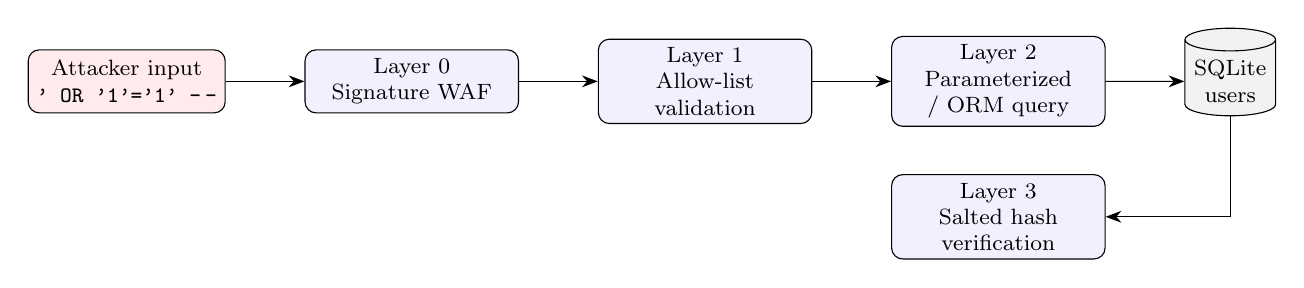
\begin{tikzpicture}[
  node distance=6mm and 10mm,
  box/.style={draw, rounded corners, align=center, minimum height=8mm, inner sep=3pt, font=\footnotesize},
  layer/.style={box, fill=blue!6, text width=2.5cm},
  db/.style={draw, cylinder, shape border rotate=90, aspect=0.25, minimum height=10mm, align=center, font=\footnotesize, fill=gray!10},
  arr/.style={-{Stealth[length=2mm]}}
]
\node[box, fill=red!8] (att) {Attacker input\\\ttfamily ' OR '1'='1' -\,-};
\node[layer, right=of att] (waf) {Layer 0\\Signature WAF};
\node[layer, right=of waf] (val) {Layer 1\\Allow-list\\validation};
\node[layer, right=of val] (bind) {Layer 2\\Parameterized\\/ ORM query};
\node[db, right=of bind] (db) {SQLite\\users};
\node[layer, below=of bind] (hash) {Layer 3\\Salted hash\\verification};
\draw[arr] (att) -- (waf);
\draw[arr] (waf) -- (val);
\draw[arr] (val) -- (bind);
\draw[arr] (bind) -- (db);
\draw[arr] (db) |- (hash);
\end{tikzpicture}
\caption{Defence-in-depth pipeline. A request must survive every enabled layer; the
defender benefits from any single layer holding.}\label{fig:arch}
\end{figure}

\subsection{The five protection variants}
\begin{description}
\item[Vulnerable baseline.] User input is concatenated into the SQL string, so the
payload is parsed as code.
\item[Variant 1 -- Parameterized query.] The statement uses \verb|?| placeholders and
binds input as data via the driver, so the payload is treated as a literal string and
never alters query structure.
\item[Variant 2 -- Allow-list validation.] The username must match
\lstinline|^[A-Za-z0-9_.@-]{1,32}$| and the password a maximum length; anything outside
the allow-list is rejected \emph{before} a query is built.
\item[Variant 3 -- ORM.] SQLAlchemy builds a parameterized statement from Python
objects, giving parameterization by construction.
\item[Variant 4 -- Credential hashing.] Passwords are stored as salted PBKDF2 hashes;
the back-end fetches by username with a parameterized query and verifies the hash in
constant time, so credentials are never compared in plaintext.
\item[Variant 5 -- Signature WAF.] A transparent rule set (tautology, comment,
stacked-query, UNION, keyword, quote-breakout, and time-based signatures) inspects each
field and blocks matches, mirroring the OWASP CRS approach of~\cite{alotaibi2023sdnwaf,floris2025modsec}
at teaching scale.
\end{description}

\section{Experimental Evaluation}\label{sec:eval}

\subsection{Protocol}
We replayed the tautology payload \lstinline|admin' OR '1'='1' -- | (with an arbitrary
password) against each mode with the WAF off and on, and separately verified that valid
credentials still authenticate under each secure mode. Success is defined as reaching
the authenticated dashboard. Query time is measured around the database call.

\subsection{Results}
Table~\ref{tab:results} reports the outcome matrix produced by the bundled
\texttt{selftest.py}. The vulnerable baseline is bypassed by the single payload; every
protection variant blocks the identical payload; and enabling the WAF additionally
blocks the request before it reaches the database even in vulnerable mode. All secure
variants continue to authenticate the legitimate \texttt{admin} account. Measured query
time stayed below 1\,ms per attempt on commodity hardware, confirming that the
secure-coding controls impose negligible overhead.

\begin{table}[htbp]
\caption{Outcome of the tautology payload against each mode (bypass = attacker reached the dashboard).}\label{tab:results}
\begin{tabular}{@{}lccc@{}}
\toprule
Mode & WAF off: bypass? & WAF on: bypass? & Legit. login \\
\midrule
Vulnerable      & \textbf{Yes} & No & --- \\
Parameterized   & No & No & OK \\
Allow-list      & No & No & OK \\
ORM             & No & No & OK \\
Hashed          & No & No & OK \\
\bottomrule
\end{tabular}
\end{table}

Figures~\ref{fig:bypass}--\ref{fig:blocked} show the demonstration. In vulnerable mode
the attacker reaches the \texttt{admin} dashboard without a password
(Fig.~\ref{fig:bypass}); under the parameterized variant the identical input is bound as
a literal parameter and rejected (Fig.~\ref{fig:blocked}).

\begin{figure}[htbp]
\centering
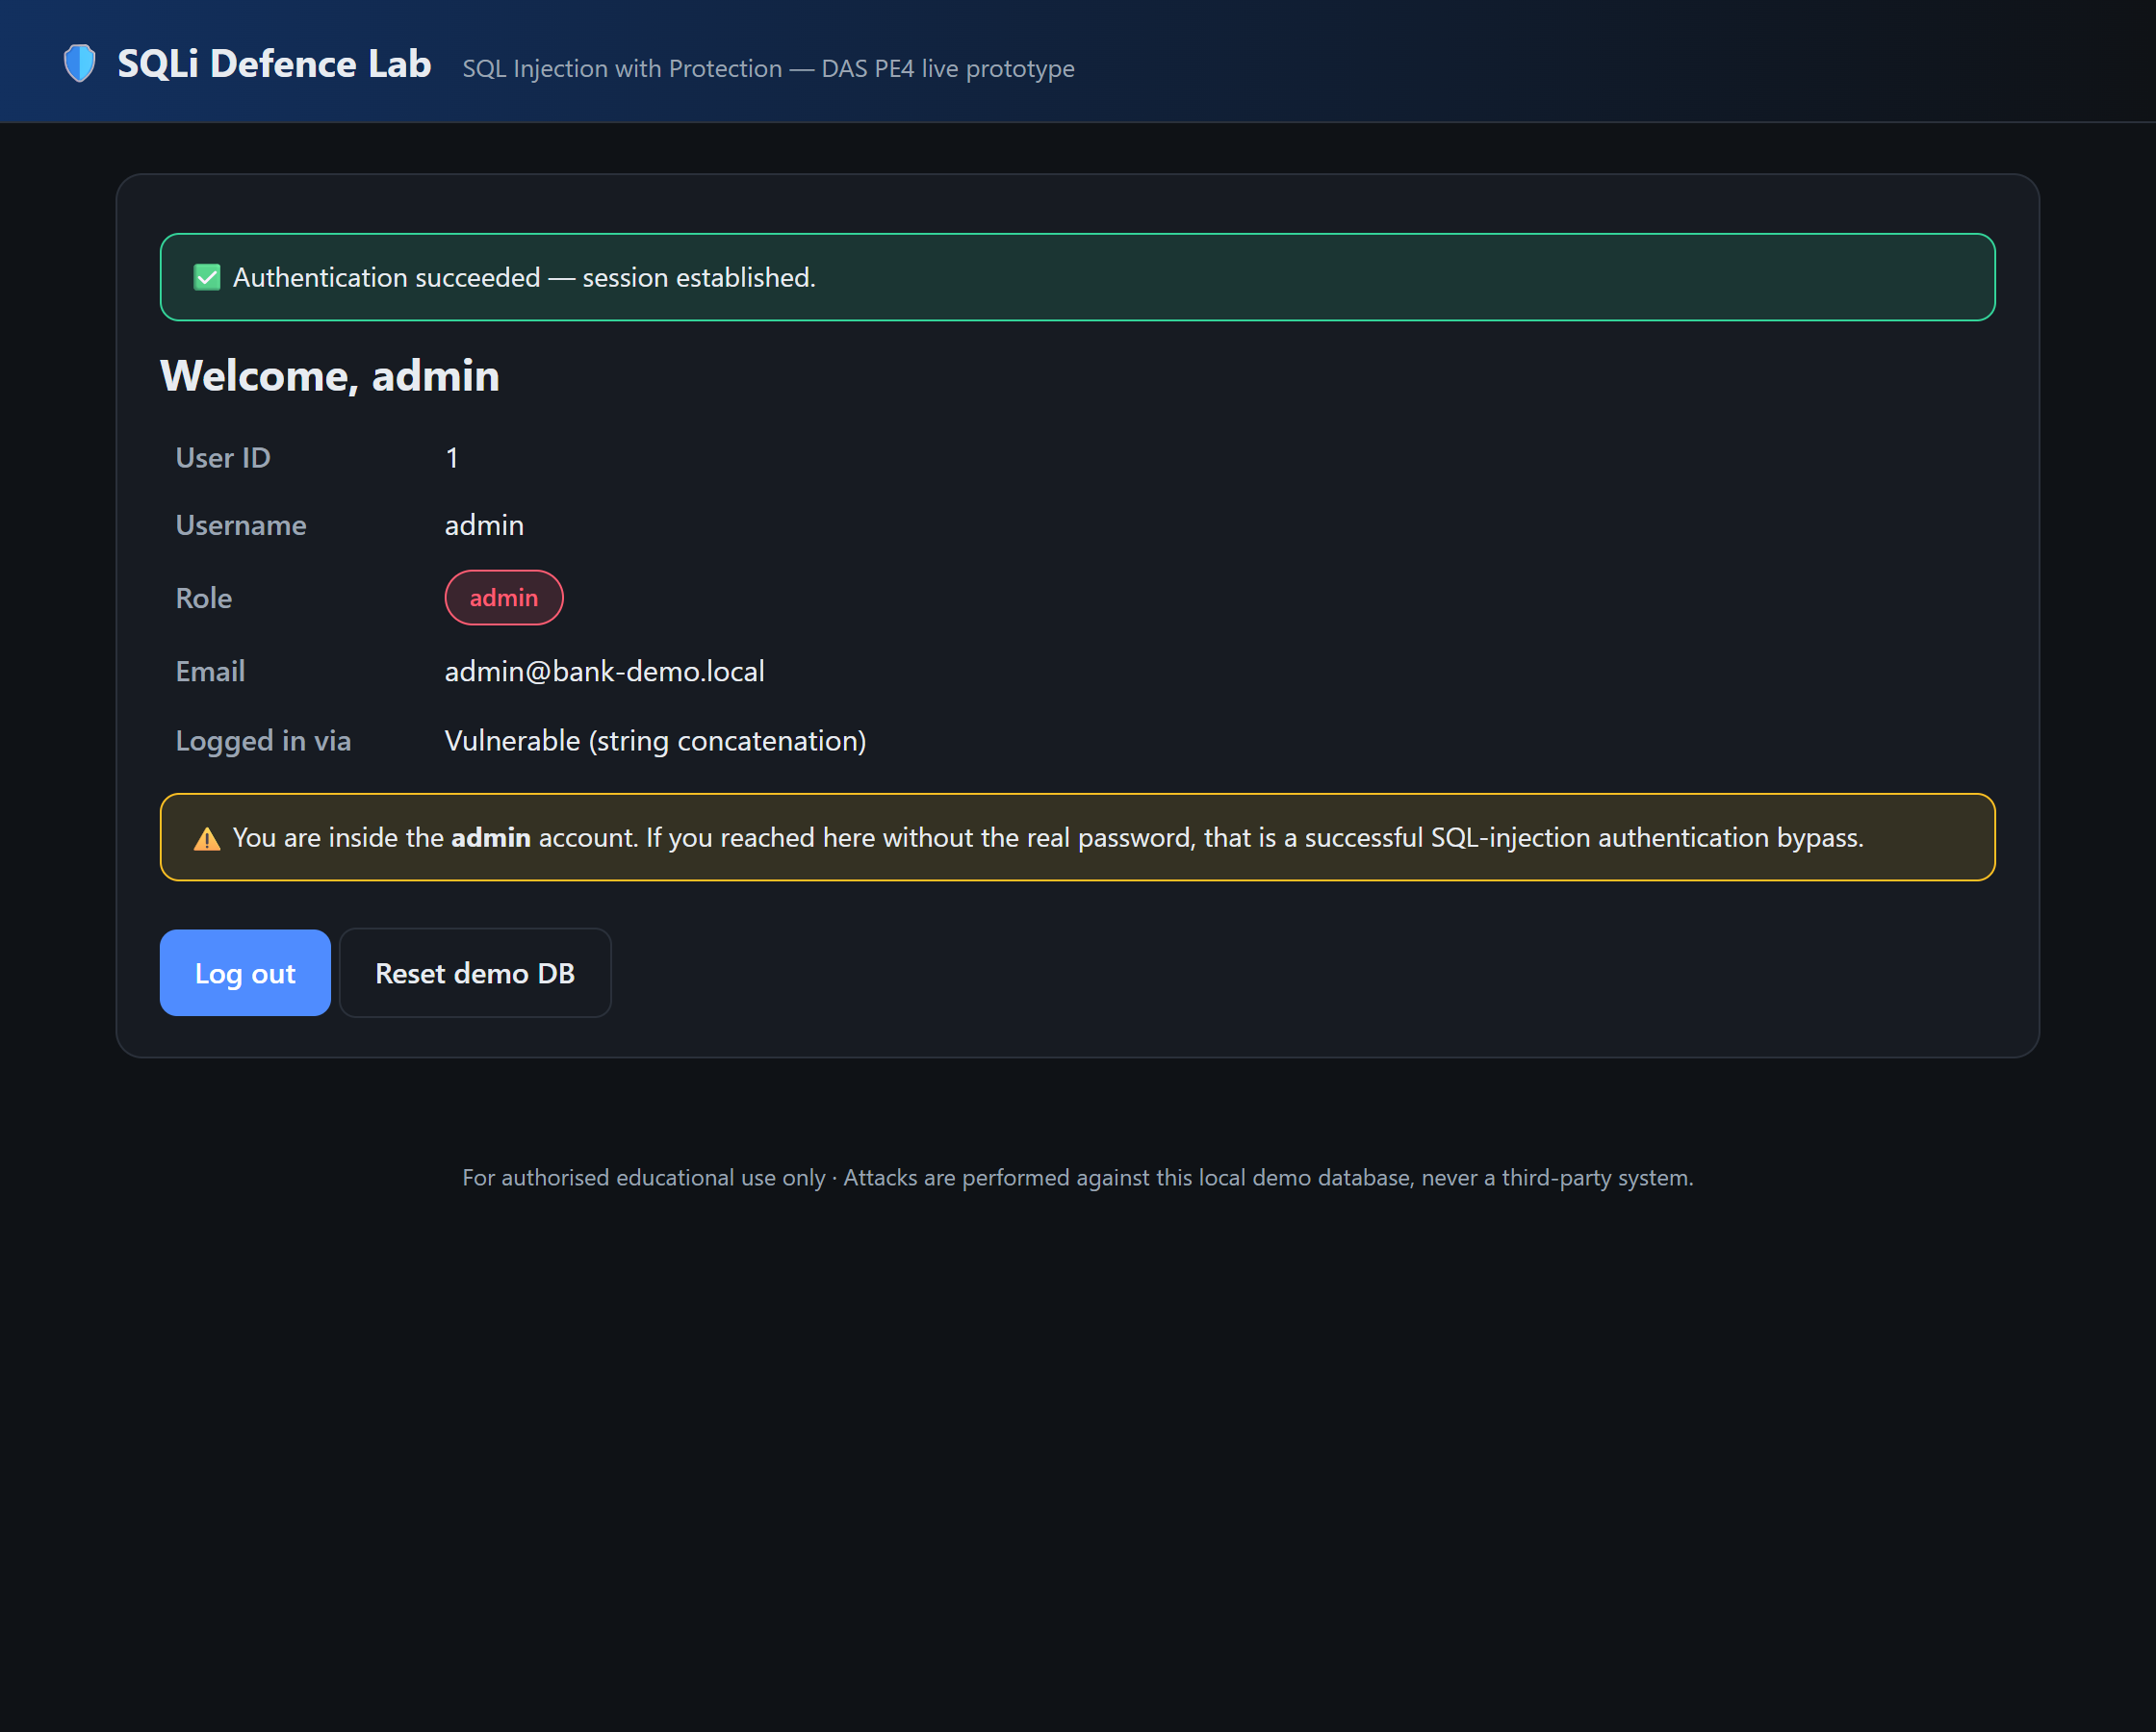
\includegraphics[width=0.86\textwidth]{fig02_vulnerable_bypass_dashboard.png}
\caption{Vulnerable baseline: the tautology payload bypasses authentication and
establishes an \texttt{admin} session.}\label{fig:bypass}
\end{figure}

\begin{figure}[htbp]
\centering
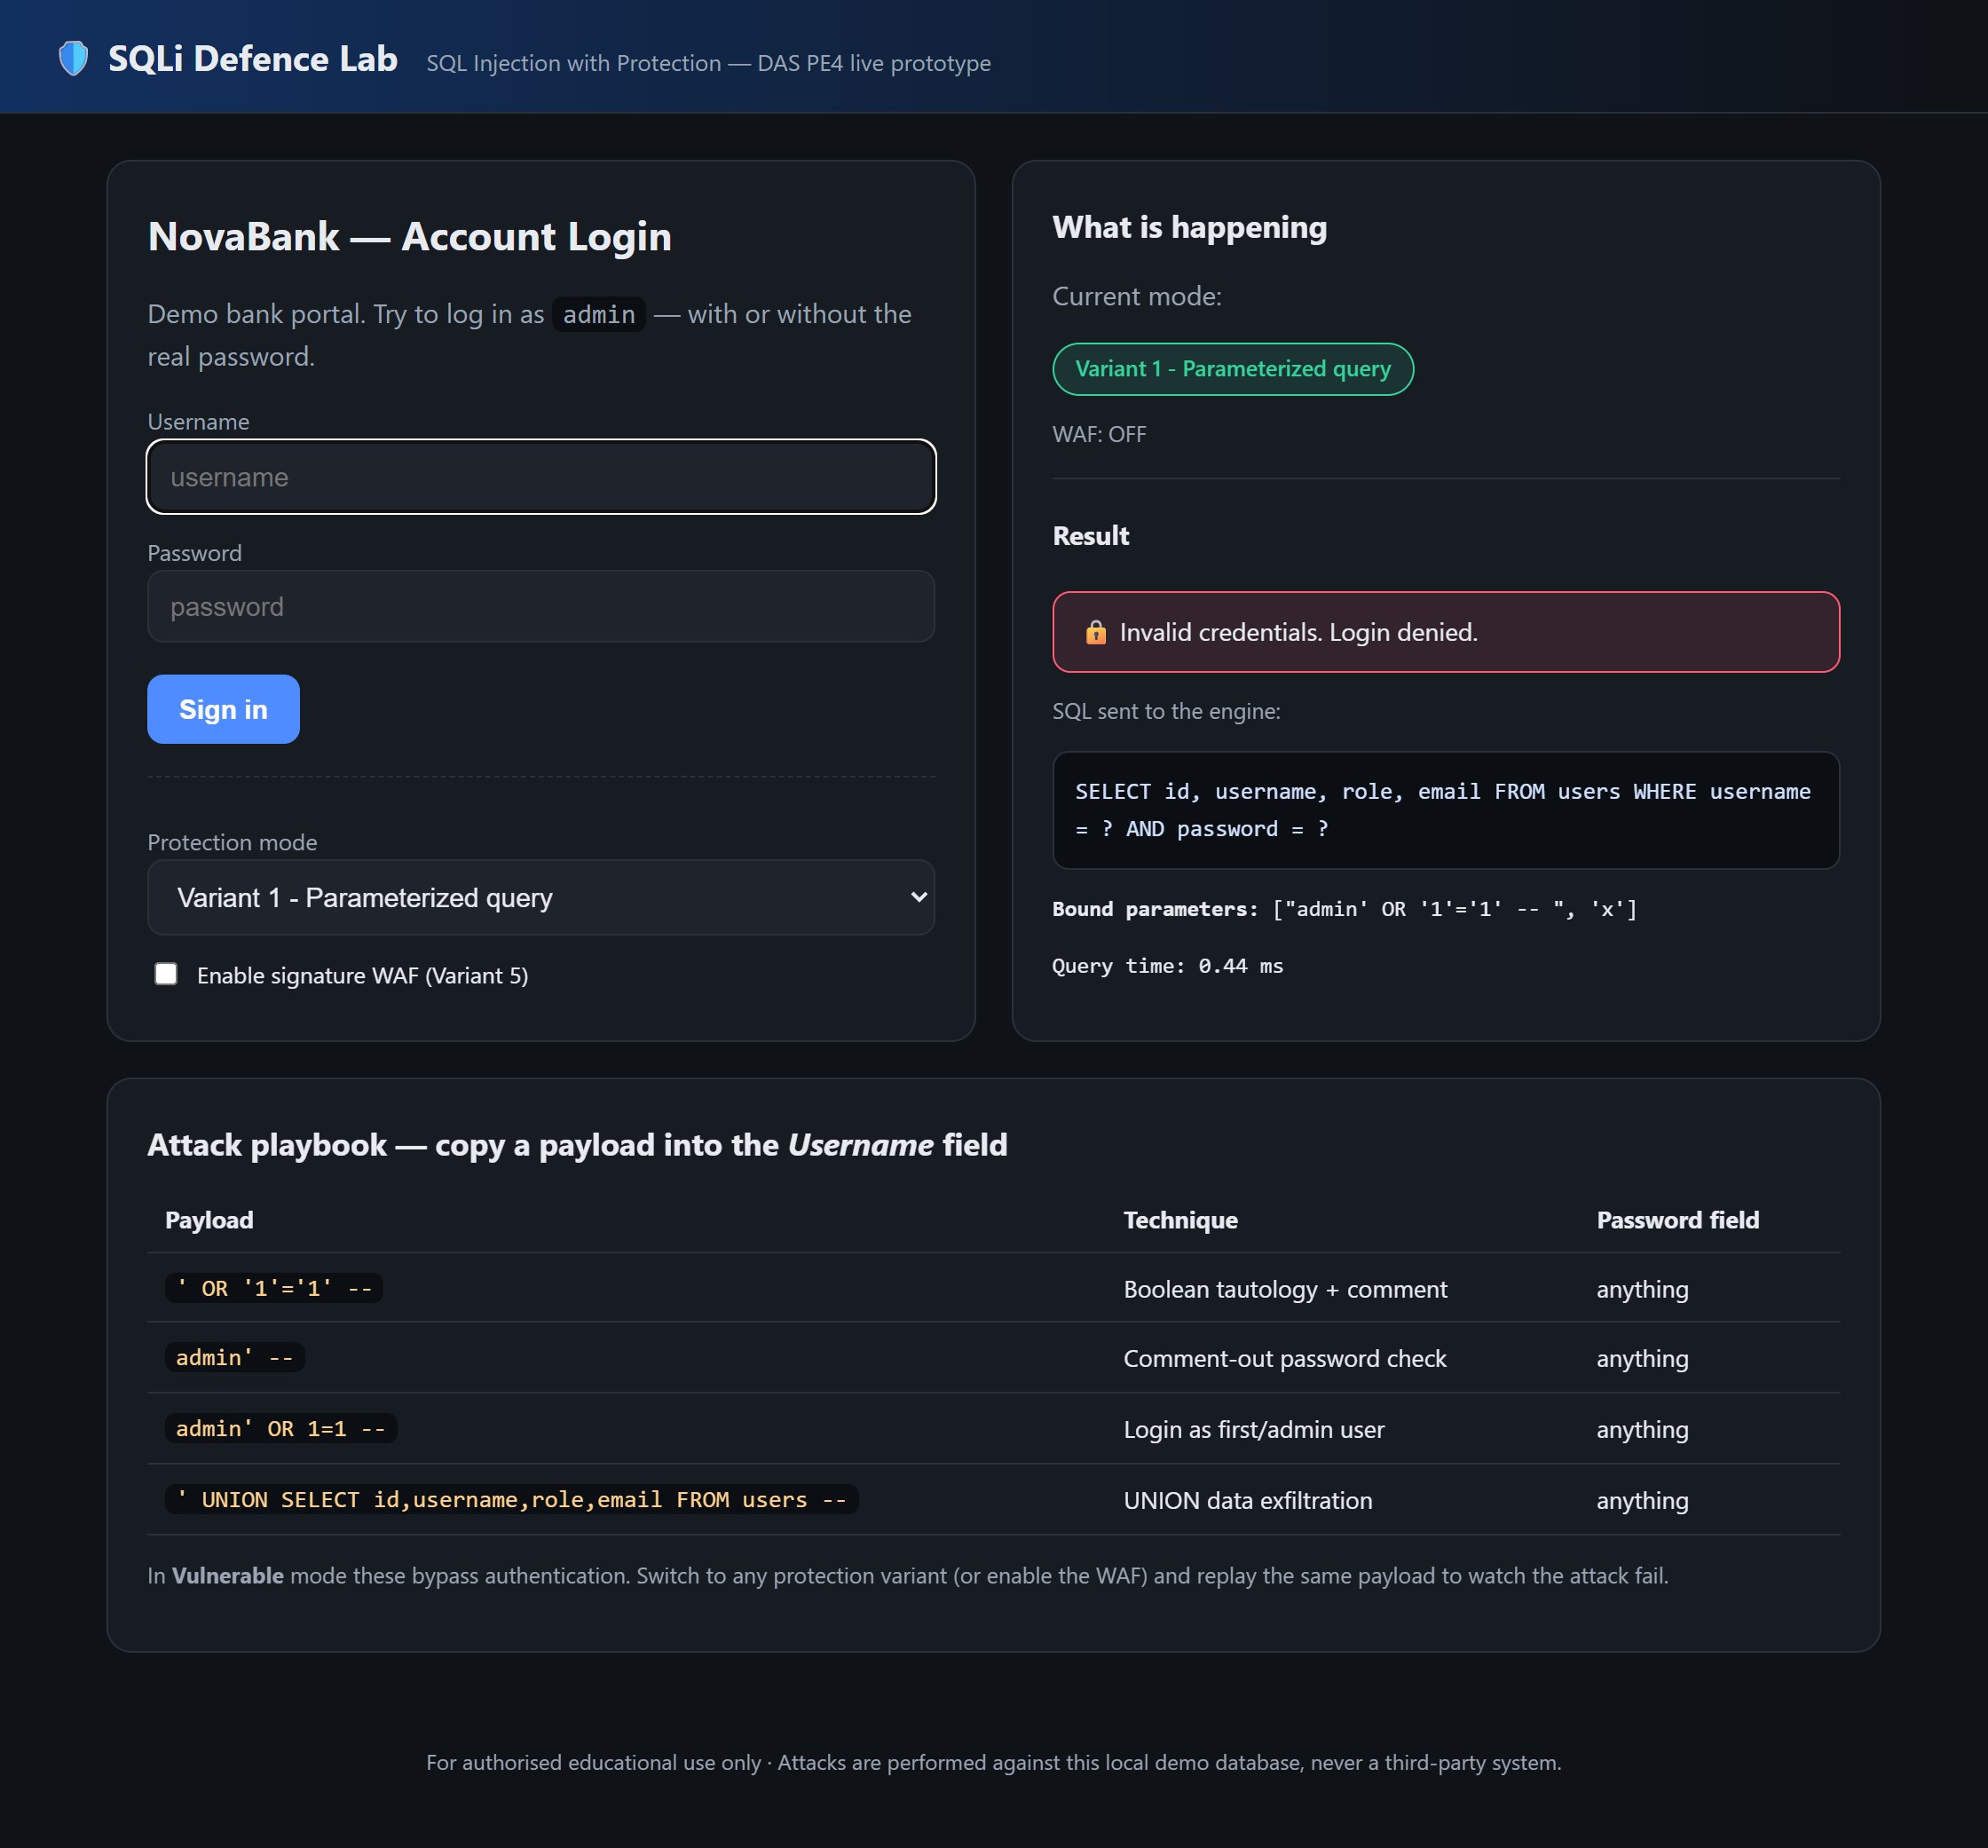
\includegraphics[width=0.86\textwidth]{fig03_parameterized_blocked.png}
\caption{Variant 1: the same payload is bound as a parameter
(\lstinline|["admin' OR '1'='1' -- ", "x"]|) and login is denied.}\label{fig:blocked}
\end{figure}

\subsection{Discussion}
The results operationalise the survey's central claim. Parameterization, ORM, and
hashing remove the root cause and are effectively free at this scale; allow-list
validation and the signature WAF add cheap, early rejection but---consistent
with~\cite{qu2024advsqli,alotaibi2023sdnwaf}---should not be relied on alone because
signatures are evadable. The strongest posture stacks a root-cause control (Variant~1
or 3) with hashing and a WAF, matching the defence-in-depth deployments
of~\cite{paul2024sqlreaper,ahmed2026deployment}.

\subsection{Ethical use and threat model}
All attacks are executed against the bundled local database only. The prototype is a
teaching artefact for authorised coursework and must not be used against systems without
explicit permission. The threat model assumes an unauthenticated attacker who controls
the login form's input fields.

\section{Conclusion and Future Work}\label{sec:conclusion}

We surveyed ten 2023--2026 studies on SQLi detection and prevention and found a field
strong on offline detection but open on adversarial robustness, generalization,
deployable prevention, and cost. We converted these gaps into a defence-in-depth login
prototype implementing five protection variants and showed empirically that each blocks
a payload that trivially defeats the vulnerable baseline, at sub-millisecond cost, while
preserving legitimate access. Future work will add an adaptive, adversarially trained
detection layer---in the spirit of~\cite{floris2025modsec}---and evaluate the stack
against mutated and blind payloads generated in the style of~\cite{qu2024advsqli},
closing the loop between secure-coding controls and learning-based defence.

\backmatter

\bmhead{Availability of code and data}
The prototype, payload battery, self-test, and screenshots are provided with this
report and are intended for authorised educational use.

\bmhead{Acknowledgements}
The authors thank the course instructor for guidance on scope and evaluation.

\bibliography{references}

\end{document}
